\section{Funktionale Anforderungen}

\subsection{Use Case-Diagramm}
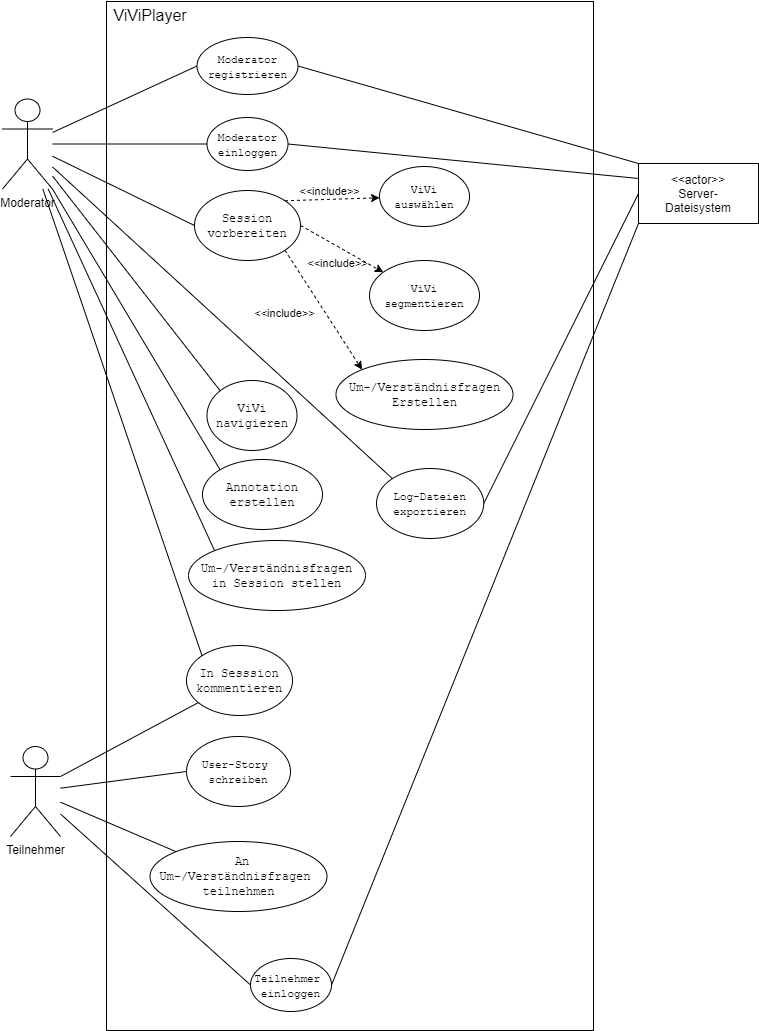
\includepdf[pages={1}]{sections/diagrams/viviplayer-uc-diagramm.pdf}
\pagebreak

\subsection{Use Case-Beschreibungen}

\subsubsection{UC: Moderator Registrieren}
\begin{tabularx}{\linewidth}{|l|X|}
	\hline
	Use Case Nr. 01			& \textbf{Moderator registrieren} \\ \hline
	Erläuterungen			& Um alle Rechte eines Moderators zu bekommen, muss ein 
							Benutzer als Moderator registriert werden. \\ \hline
	Systemgrenzen (Scope)	& Registrierung-System. \\ \hline
	Ebene					& Hauptfunktion \\ \hline
	Vorbedingung			& Die Web-App ist betriebsbereit. Der Benutzer befindet sich auf die 
							  Hauptseite von ViViPlayer-Web-App. \\ \hline
	Mindestgarantie			& Im Fehlerfall wird kein neues Moderator-Konto im System 
	                          registriert. Klare Fehlermeldung wird ausgegeben. \\ \hline
	Erfolgsfall  			& Ein neues Moderator-Konto wurde erstellt. \\ \hline
	Stakeholder				& Systembediener (Moderator) - möchte die Funktionen der Web-App so 
							  schnell wie möglich nutzen. \\
							& Systembesitzer (Systemadministrator) - möchte, dass die Funktionen 
							  der Web-App für die Benutzer mit korrekten Zugriffsrechten verfügbar sind.\\ \hline
	Hauptakteur				& Systembediener (Moderator) \\ \hline
	Auslöser				& Der Benutzer klickt auf den ``Registrieren''-Button. \\ \hline	
	Hauptszenario			& 1. Der Benutzer klickt auf den ``Registrieren''-Button. \\
							& 2. Das System fordert den Benutzer auf, eine Email-Adresse 
							  sowie die Passwort für das neue Konto einzugeben. \\
							& 3. Der Benutzer gibt seinen Benutzername und seine Passwort 
							  ein und bestätigt sie \\
							& 4. Das System und ein anderer Moderator validiert die vom 
							  Benutzer eingegebene Daten. Eine Meldung wird als 
							  Anleitung angezeigt, was der neue Benutzer weiter machen soll. \\
							& 5. Der Benutzer wird zurück zur Hauptseite geleitet. 
							  \\ \hline
	Erweiterungen			& 4a. WENN das System feststellt, dass die eingegebene Daten 
							  (Benutzername und Passwort) nicht gültig sind, DANN wird eine Fehlermeldung ausgegeben. Zurück zu Schritt 2. \\ \hline
	Priorität				& niedrig \\ \hline
	Verwendungshäufigkeit	& weniger häufig \\ \hline
\end{tabularx}

\\[0.5cm]
\pagebreak

\subsubsection{UC: Moderator Einloggen}
\begin{tabularx}{\linewidth}{|l|X|}
	\hline
	Use Case Nr. 02			& \textbf{Moderator einloggen} \\ \hline
	Erläuterungen			& Der Benutzer möchte sich als Moderator einloggen, damit er eine 
							  Session im ViViPlayer abhalten kann. \\ \hline
	Systemgrenzen (Scope)	& Login-System \\ \hline
	Ebene					& Hauptfunktion \\ \hline
	Vorbedingung			& Die Web-App ist betriebsbereit. Der Benutzer befindet sich auf
							  Hauptseite der Web-App. \\ \hline
	Mindestgarantie			& Das Einloggen des Benutzers wird abgesagt, falls der eingegebene
							  Benutzername/die Email-Adresse nicht im Datenbank oder die Passwort falsch ist. Eine Fehlermeldung wird dann ausgegeben.
							  \\ \hline
	Erfolgsfall 			& Der Zugriff des Benutzers wurde erfolgreich bestätigt. Der
							  Benutzer befindet sich auf der Moderator-Hauptseite. 
							  \\ \hline
	Stakeholder				& Systembediener (Moderator) - möchte die Funktionen der Web-App 
							  schnell wie möglich nutzen. \\
							& Systembesitzer (Systemadministrator) - möchte, dass die Funktionen 
							  der Web-App für die Benutzer mit korrektem Zugriffsrecht verfügbar sind.\\ \hline
	Hauptakteur				& Systembediener (Moderator) \\ \hline
	Auslöser				& Der Benutzer klickt auf die ``Einloggen als Moderator''-Option.\\ 
							  \hline	
	Hauptszenario			& 1. Der Benutzer klickt auf die ``Einloggen als 
							  Moderator''-Option.\\
							& 2. Das System zeigt das Moderator-Loginsformular an. \\
							& 3. Der Benutzer gibt sein Benutzername/seine Email-Adresse und 
							  seine Passwort ein. \\
							& 4. Das System validiert die vom Benutzer eingegebene
							  Log-in-Daten. \\
							& 5. Der Benutzer wird im System angemeldet und weiter zur
							  Moderator-Hauptseite geleitet. \\ \hline
	Erweiterungen			& 1a. WENN das System feststellt, dass die eingegebene Daten 
							  (Benutzername/Email-Adresse und Passwort) nicht abgestimmt sind, DANN wird eine Fehlermeldung ausgegeben. Zurück zu Schritt 2. \\ \hline
	Priorität				& mittel \\ \hline
	Verwendungshäufigkeit	& häufig \\ \hline
\end{tabularx}

\\[0.5cm]
\pagebreak

\subsubsection{UC: Teilnehmer Einloggen}
\begin{tabularx}{\linewidth}{|l|X|}
	\hline
	Use Case Nr. 03			& \textbf{Teilnehmer Einloggen} \\ \hline
	Erläuterungen			& Damit ein Teilnehmer alle Funktionen der App benutzen kann, 
							  muss er sein Zugriffsrecht via TAN bestätigen. \\ \hline
	Systemgrenzen (Scope)	& Login-System \\ \hline
	Ebene					& Hauptebene \\ \hline
	Vorbedingung			& Die Web-App ist betriebsbereit. Der Benutzer befindet sich in
							  Hauptseite der Web-App \\ \hline
	Mindestgarantie			& Das Log-in des Benutzers wird abgesagt, falls die eingegebene
							  TAN nicht richtig ist. Eine Fehlermeldung wird ausgegeben
							  \\ \hline
	Erfolgsfall 			& Der Zugriff des Benutzers wurde erfolgreich bestätigt. Der
							  Benutzer hat sich auf der Moderator-Hauptseite befindet. \\ \hline
	Stakeholder				& Systembediener - möchte die Funktionen der Web-App schnell 
							  wie möglich nutzen. \\
							& Herr Jianwei Shi (Systembesitzer) - möchte die Funktionen der 
							  Web-App für die Benutzer mit korrektem Zugriffsrecht verfügbar sein.\\ \hline
	Hauptakteur				& Systembediener, die Teilnehmer-Rechte haben möchten \\ \hline
	Auslöser				& Der Benutzer möchte an einem Session des ViViPlayer
							  teilnehmen. Er befindet sich auf der Hauptseite der Web-App,
							  um mit TAN einzuloggen. \\ \hline	
	Hauptszenario			& 1. Der Benutzer befindet sich auf der Hauptseite der Web-App,
	                          um mit TAN einzuloggen. \\
	                        & 2. Das System fordert den Benutzer auf, als Teilnehmer eine
							  TAN einzugeben. \\
							& 3. Der Benutzer gibt seine vom Moderator erhaltene TAN ein. \\
							& 4. Das System validiert die vom Benutzer eingegebene
							  TAN. \\
							& 5. Dem Benutzer wird im System angemeldet und weiter zur
							  Teilnehmer-Hauptseite geleitet. \\ \hline
	Erweiterungen			& 4a. Wenn das System feststellt, dass die eingegebene TAN nicht 
							  eine von System generierte TAN ist, wird eine Fehlermeldung 
							  ausgegeben. Das System geht zurück zu Schritt 2. \\ \hline
	Priorität				& mittel \\ \hline
	Verwendungshäufigkeit	& sehr häufig \\ \hline
\end{tabularx}

\\[0.5cm]
\pagebreak

\subsubsection{UC: Moderator Session-Vorbereiten}
\begin{tabularx}{\linewidth}{|l|X|}
	\hline
	Use Case Nr. 04			& \textbf{Session vorbereiten} \\ \hline
	Erläuterungen			& Bevor ein Moderator eine Session mit den Teilnehmer anfangen 
	                          kann, muss er zuerst vorbereiten. Das heißt: er muss das ViVi einbetten und segmentieren, Verständnisfragen vorbereiten und TAN für die Session erzeugen. \\ \hline
	Systemgrenzen (Scope)	& Gesamtsystem. \\ \hline
	Ebene					& Hauptfunktion. \\ \hline
	Vorbedingung			& Die Web-App ist betriebsbereit. Der Benutzer hat 
	                          Moderator-Rechte. Er wählt die Option, eine neue Session zu erstellen, von der Moderator-Hauptseite. \\ \hline
	Mindestgarantie			& Im Fehlerfall wird keine Session erstellt.\\ \hline
	Erfolgsfall  			& Das segmentierte Vision-Video sowie eine sichere TAN sind 
	                          bereitgestellt für eine ViViPlayer-Session. \\ \hline
	Stakeholder				& Systembediener (Moderator) - will eine produktive Session mit den 
	                          Teilnehmer via ViViPlayer. \\
							& Systembesitzer (Herr Jianwei Shi) - möchte, dass alle Sessions 
							  in der Web-App erfolgreich durchgeführt werden. \\ \hline
	Hauptakteur				& Systembediener (Moderator). \\ \hline
	Auslöser				& Der Benutzer klickt auf die "Session erstellen"-Option. \\ \hline	
	Hauptszenario			& 1. Der Benutzer klickt auf die "Session erstellen"-Option. \\ 
							& 2. Das System zeigt die ViVi-Auswählen-Oberfläche an. \\
							& 3. Der Benutzer wählt ein ViVi und bestätigt. (UC 5) \\ 
							& 4. Das System zeigt die ViVi-Segmentieren-Oberfläche. \\ 
							& 5. Der Benutzer segmentiert das von ihm ausgewählte Video und 
							  bestätigt. (UC 6) \\
							& 6. Das System zeigt die Frage-Vorbereiten-Oberfläche. \\
							& 7. Der Benutzer bereitet die Um-/Verstänisfragen vor und bestätigt.
							  (UC 7) \\
							& 8. Das System zeigt die ViVi-Überblick-Oberfläche. \\ 
							& 9. Der Benutzer prüft noch mal alle Vorbereitungschritte und 
							  klickt auf das "Erstellen"-Button. \\
							& 10. Das System erstellt eine neue Session und eine sichere TAN. \\ 
							  \hline
	Erweiterungen			& 4a. WENN das Video nicht eingebettet werden kann, DANN wird eine 
	                          Fehlermeldung gezeigt. Zurück zu Schritt 2. \\
							& 6a. WENN die Segmentierung nicht gültig ist, DANN wird eine 
							  Fehlermeldung ausgegeben. Zurück zu Schritt 4.\\
							& 8a. WENN es Fehler bei der Eingabe der Fragen, DANN wird 
							  eine Fehlermeldung ausgegeben. Zurück zu Schritt 4. \\ \hline
	Priorität				& hoch \\ \hline
	Verwendungshäufigkeit	& häufig \\ \hline
\end{tabularx}
\\[0.5cm]
\textbf{Erläuterungen und Details}
\begin{itemize}
	\item ViVi: die Abkürzung von dem Begriff ``Vision-Video''.
	\item ViVi-Auswählen-Oberfläche: Eine Menge von ViVis werden hier angezeigt, damit der Benutzer eines davon auswählen kann.
	\item ViVi-Segmentieren-Oberfläche: da gibt es ein Video-Fenster mit Controller, eine Liste von Segmenten mit ihrem Namen und Zeitstempeln sowie ein Button zum Hinzufügen der neuen Segmente. 
	\item Frage-Vorbereiten-Oberfläche: es gibt eine Liste von erstellten Fragen
	sowie ein Fenster zum Bearbeitung einer neuen Frage.
	\item TAN-Oberfläche: man kann entweder manuell oder automatisch TAN für die Session hier erzeugen.
	\item ViVi-Überblick-Oberfläche: hier kann der Benutzer seine schon eingegebene Konfiguration nachschauen, um Fehler zu checken.
	\item Für die ViVi-Auswählen-, ViVi-Segmentieren-, TAN- und ViVi-Überblick-Oberfläche gibt es möglich ein ``Zurück''-Button, damit man nach Wunsch modifizieren kann.
\end{itemize}
\pagebreak

\subsubsection{UC: Moderator ViVi Auswählen}
\begin{tabularx}{\linewidth}{|l|X|}
	\hline
	Use Case Nr. 05			& \textbf{ViVi auswählen} \\ \hline
	Erläuterungen			& Vision-Video auswählen ist der erste Schritt zur Vorbereitung 
							  einer ViViPlayer-Session. \\ \hline
	Systemgrenzen (Scope)	& Gesamtsystem. \\ \hline
	Ebene					& Hauptebene \\ \hline
	Vorbedingung			& Die Web-App ist betriebsbereit. Der Benutzer hat 
							  Moderator-Rechte. Er wählt die Option, eine neue Session zu 
							  erstellen, auf der Moderator-Hauptseite. \\ \hline
	Mindestgarantie			& Im Fehlerfall wird kein Video ausgewählt und somit keine 
							  Session.\\ \hline
	Erfolgsfall 			& Der Benutzer konnte sein gewünschtes Video problemlos auswählen. 
							  \\ \hline
	Stakeholder				& Systembediener (Moderator) - will eine produktive Session mit den 
							  Teilnehmer via ViViPlayer. \\
							& Systembesitzer (Herr Jianwei Shi) - möchte alle Sessions in der 
							  Web-App erfolgreich durchgeführt werden. \\ \hline
	Hauptakteur				& Systembediener (Moderator). \\ \hline
	Auslöser				& Der Benutzer klickt auf die "Session erstellen"-Option. \\ \hline	
	Hauptszenario			& 1. Der Benutzer klickt auf die "Session erstellen"-Option. \\
							& 2. Das System zeigt die ViVi-Auswählen-Oberfläche an. \\
							& 3. Der Benutzer kann ein ViVi vom Server-Dateisystem auswählen 
							  und klickt auf das ``Weiter''-Button, wenn er fertig ist. \\
							& 4. Das System zeigt die ViVi-Segmentieren-Oberfläche an. \\ \hline
	Erweiterungen			& 3a. Alternativ kann das Video via Pfad eingebettet werden. \\ 
							& 4a. WENN das Video nicht ausgewählt werden kann, DANN wird eine 
							  Fehlermeldung gezeigt. Zurück zu Schritt 2. \\ \hline
	Priorität				& sehr hoch \\ \hline
	Verwendungshäufigkeit	& häufig \\ \hline
\end{tabularx}
\\[0.5cm]
\pagebreak

\subsubsection{UC: Moderator ViVi Segmentieren}
\begin{tabularx}{\linewidth}{|l|X|}
	\hline
	Use Case Nr. 06			& \textbf{Moderator Vision-Video Segmentieren} \\ \hline
	Erläuterungen			& Vision-Video segmentieren ist der zweite Schritt zur 
							  Vorbereitung einer ViViPlayer-Session. \\ \hline
	Systemgrenzen (Scope)	& Applikation. \\ \hline
	Ebene					& Hauptebene \\ \hline
	Vorbedingung			& Die Web-App ist betriebsbereit. Der Benutzer hat Moderator-Rechten \\ \hline
	Mindestgarantie			& Im Fehlerfall wird das Video nicht segmentiert. \\ \hline
	Erfolgsgarantie			& Das ViVi wird erfolgreich segmentiert. \\ \hline
	Stakeholder				& Der Benutzer - will eine produktive Session mit den Teilnehmer via
							  ViViPlayer. \\
							& Herr Jianwei Shi - möchte alle Sessions in der Web-App erfolgreich durchgeführt
							  werden. \\ \hline
	Hauptakteur				& Der Benutzer \\ \hline
	Auslöser				& Der Benutzer hat schon ein ViVi ausgewählt und klick auf ``Weiter''-Button. 
							  \\ \hline	
	Hauptszenario			& 1. Das System zeigt ViVi-Segmentieren-Oberfläche. \\
							& 2. Von dem Video-Fenster spielt der Benutzer das Video ab, bis zu seinem
							  gewünschten Zeitstempel für ein neues Segment, danach benennt er das Segment nach 
							  seinem Wunsch und klickt ``Hinzufügen''. \\
							& 3. Das System fügt das neue Segment in der Segmente-Liste hinzu. \\
							& 4. Der Benutzer klickt auf ``Weiter''-Button. \\
							& 5. Das System zeigt Verständnisfrage-Vorbereiten-Oberfläche   
							  an. \\ \hline
	Erweiterung				& 2a. Alternativ kann der Benutzer die automatische 
							  Segmentierung nutzen. \\
							& 3a. Wenn der Benutzer noch nicht fertig mit dem Segmentierung 
							  ist, geht der Benutzer zurück zu Schritt 2. \\ 
							& 3b. Falls der Name eines Segments leer oder eine Zeitstempel 
							  nicht gültig ist, wird eine Fehlermeldung ausgegeben. Kein neues Segment wird hinzugefügt. \\ \hline
	Priorität				& sehr hoch \\ \hline
	Verwendungshäufigkeit	& häufig \\ \hline
\end{tabularx}
\\[0.5cm]
\textbf{Erläuterungen und Details}
\begin{itemize}
	\item Shot: Ein anonymer Begriff für Segment.
\end{itemize}
\pagebreak

\subsubsection{UC: Moderator Fragen Erstellen}
\begin{tabularx}{\linewidth}{|l|X|}
	\hline
	Use Case Nr. 07			& \textbf{Um-/Verstänisfragen erstellen} \\ \hline
	Erläuterungen			& Um-/Verstänisfragen erstellen ist der dritte Schritt zur 
							  Vorbereitung einer ViViPlayer-Session. \\ \hline
	Systemgrenzen (Scope)	& Gesamtsystem. \\ \hline
	Ebene					& Hauptfunktion. \\ \hline
	Vorbedingung			& Die Web-App ist betriebsbereit. Der Benutzer hat Moderator
							  -Rechte und schon ein ViVi ausgewählt (UC 5) und segmentiert (UC 6). Er befindet sich auf der ViVi-Segmentieren-Seite. \\ \hline
	Mindestgarantie			& Im Fehlerfall wird die Um-/Verstänisfragen nicht erstellt. Das ViVi 
							  bleibt unverändert. \\ \hline
	Erfolgsfall    			& Eine Liste von Verständnisfragen ist erfolgreich hinzugefürgt.
							  \\ \hline
	Stakeholder				& Systembediener (Moderator) - will eine produktive Session mit 
							  anderen Benutzer via ViViPlayer. \\
							& Systembesitzer (Herr Jianwei Shi) - möchte, dass alle Sessions 
							  in der Web-App erfolgreich durchgeführt werden können. \\ \hline
	Hauptakteur				& Systembediener (Moderator). \\ \hline
	Auslöser				& Der Benutzer klickt auf den ``Weiter''-Button. \\ \hline	
	Hauptszenario			& 1. Der Benutzer klickt auf den ``Weiter''-Button. \\  
							& 2. Das System zeigt die Frage-Vorbereiten-Oberfläche. \\
							& 3. Der Benutzer tippt neue Frage, die Auswahlen für die 
							  Frage, sowie den Zeitstempel und den Typ der Frage ein und 
							  bestätigt. \\ 
							& 4. Das System fügt die neue Verstänis-/Umfrage in der Liste 
							  hinzu. \\ 
							& 5. Der Benutzer klickt auf den ``Weiter''-Button. \\ 
							& 6. Das System zeigt die TAN-Oberfläche an. \\ \hline
	Erweiterungen			& 4a. WENN die Frage leer ist oder es keine Auswahl für die 
							  Frage gibt oder der Zeitstempel nicht gültig ist, DANN wird eine 
							  Fehlermeldung angezeigt. Zurück zu Schritt 2. \\ 
							& 5a. WENN der Benutzer noch nicht fertig mit der 
							  Fragen-Vorbereitung ist, DANN geht er zurück zu Schritt 3. \\ \hline
	Priorität				& mittel \\ \hline
	Verwendungshäufigkeit	& normal \\ \hline
\end{tabularx}
\\[0.5cm]
\pagebreak

\subsubsection{UC: Moderator TAN Erzeugen}
\begin{tabularx}{\linewidth}{|l|X|}
	\hline
	Use Case Nr. 08			& \textbf{Moderator TAN für ViViPlayer-Session Erzeugen} \\ \hline
	Erläuterungen			& TAN erzeugen ist der letzte Schritt zur Vorbereitung einer 
							  ViViPlayer-Session. Danach kann die Teilnehmer mit TAN einloggen. \\ \hline
	Systemgrenzen (Scope)	& Gesamtsystem. \\ \hline
	Ebene					& Hauptfunktion. \\ \hline
	Vorbedingung			& Die Web-App ist betriebsbereit. Der Benutzer hat Moderator-
							  Rechte und schon ein ViVi ausgewählt (UC 3.2.5), segmentiert (UC 3.2.6) sowie eine Liste von Fragen hinzugefügt (UC 3.2.7), und klickt auf ``Weiter''. \\ \hline
	Mindestgarantie			& Im Fehlerfall wird keine TAN sowie keine Session erstellt.
							  \\ \hline
	Erfolgsfall 			& Eine sichere TAN ist für die Session erstellt. \\ \hline
	Stakeholder				& Systembediener - will eine produktive Session mit den Teilnehmer 
							  via ViViPlayer. \\
							& Herr Jianwei Shi (Systembesitzer) - möchte alle Sessions in der 
							  Web-App erfolgreich durchgeführt werden. \\ \hline
	Hauptakteur				& Systembediener mit Moderator-Rolle. \\ \hline
	Auslöser				& Der Benutzer befindet sich auf der ViVi-Fragen-Vorbereiten-Seite 
	                          und klickt auf ``Weiter''. \\ \hline	
	Hauptszenario			& 1. Der Benutzer befindet sich auf ViVi-Fragen-Vorbereiten-Seite
							  und klickt auf ``Weiter''. \\
							& 2. Das System zeigt TAN-Oberfläche. \\
							& 3. Der Benutzer erzeugt eine neue TAN für die Session, und klickt 
							  auf das ``Weiter''-Button. \\ 
							& 4. Das System zeigt ViVi-Überblick-Oberfläche an. \\ \hline
	Erweiterungen			& 3a. Alternativ kann man die automatische TAN-Erzeugung nutzen. 
							  \\
							& 3b. Wenn die TAN nicht sicher genug ist, wird eine Fehlermeldung 
							  ausgegeben. Das System geht zurück zu Schritt 2. \\ \hline
	Priorität				& hoch \\ \hline
	Verwendungshäufigkeit	& häufig \\ \hline
\end{tabularx}
\\[0.5cm]
\pagebreak

\subsubsection{UC: Moderator ViVi Navigieren}
\begin{tabularx}{\linewidth}{|l|X|}
	\hline
	Use Case Nr. 09			& \textbf{Moderator Vision-Video navigieren} \\ \hline
	Erläuterungen			& Als Moderator kann der Benutzer das ViVi navigieren. \\ \hline
	Systemgrenzen (Scope)	& Gesamtsystem. \\ \hline
	Ebene					& Hauptfunktion. \\ \hline
	Vorbedingung			& Die Web-App ist betriebsbereit. Der Benutzer hat Moderator-
							  Rechte und hat schon eine ViViPlayer-Session erstellt (UC 3.2.5, UC 3.2.6, UC 3.2.7, UC 3.2.8). Der ist in einer Session mit anderen Benutzern, die entweder Moderator oder Teilnehmer sind. \\ \hline
	Mindestgarantie			& Im Fehlerfall wird das ViVi beim Moderator oder bei Teilnehmer 
							  nicht navigiert. Das ViVi steht noch in der ViViPlayer-Oberfläche 
							  und wird nicht gelöscht oder verloren. \\ \hline
	Erfolgsfall 			& Das ViVi wurde für alle Benutzer in der Session navigiert. 
							  \\ \hline
	Stakeholder				& Systembediener - will eine produktive Session mit den Teilnehmer 
							  via ViViPlayer. \\
							& Herr Jianwei Shi (Systembesitzer) - möchte alle Sessions in der 
							  Web-App erfolgreich durchgeführt werden. \\ \hline
	Hauptakteur				& Systembediener mit Moderator-Rolle. \\ \hline
	Auslöser				& Der Benutzer navigiert das Video zu seinem gewünschten 
							  Zeitpunkt. \\ \hline	
	Hauptszenario			& 1. Der Benutzer navigiert das Video zu seinem gewünschten 
							  Zeitpunkt. \\
							& 2. Das System erkennt die Navigation von dem Benutzer, und 
							  schickt ein Signal zu allen anderen Benutzer. \\ 
							& 3. Das ViVi wird für alle Benutzer in der Session navigiert. 
							  \\ \hline
	Erweiterungen			&  \\ \hline
	Priorität				& sehr hoch \\ \hline
	Verwendungshäufigkeit	& sehr häufig \\ \hline
\end{tabularx}
\\[0.5cm]
\pagebreak

\subsubsection{UC: Moderator Umfragen Erstellen}
\begin{tabularx}{\linewidth}{|l|X|}
	\hline
	Use Case Nr. 09			& \textbf{Moderator Umfrage Erstellen} \\ \hline
	Erläuterungen			& Als Moderator kann der Benutzer mehrere Umfragen während der Session 
							  erstellen, um Feedbacks von Teilnehmer zu bekommen. \\ \hline
	Systemgrenzen (Scope)	& Applikation. \\ \hline
	Ebene					& Hauptebene. \\ \hline
	Vorbedingung			& Die Web-App ist betriebsbereit. Der Benutzer hat Moderator-
							  Rechten. \\ \hline
	Mindestgarantie			& Keine Umfrage wird erstellt. \\ \hline
	Erfolgsgarantie			& Die Umfrage wird erstellt, alle Teilnehmer können die sehen und 
							  interagieren\\ \hline
	Stakeholder				& Der Benutzer - will eine produktive Session mit den Teilnehmer 
							  via ViViPlayer. \\
							& Herr Jianwei Shi - möchte alle Sessions in der Web-App 
							  erfolgreich durchgeführt werden. \\ \hline
	Hauptakteur				& Der Benutzer. \\ \hline
	Auslöser				& Der Benutzer ist in einer Session mit anderen Benutzern, die 
							  können entweder Moderator oder Teilnehmer. \\ \hline	
	Hauptszenario			& 1. Der Benutzer klickt auf ``Umfrage''-Tab. \\
							& 2. Das System zeigt ein neues Eingabe-Feld an. \\ 
							& 3. Der Benutzer gibt die Umfrage und Zeitraum für die ein und bestätigt. 
							  \\
							& 4. Das System zeigt die Umfrage für alle Teilnehmer an. \\ 
							& 5. Alle Teilnehmer antworten die Umfrage. \\
							& 6. Nach dem Zeitraum zeigt das System ein Balkendiagramm als Ergebnis. 
							  \\ \hline
	Erweiterung				& 3a. Wenn es keine Frage-Texte oder keine Auswahl für die Umfrage gibt,
							  zeigt das System eine Fehlermeldung an. \\ \hline
	Priorität				& mittel \\ \hline
	Verwendungshäufigkeit	& normal \\ \hline
\end{tabularx}
\\[0.5cm]
\pagebreak

\subsubsection{UC: User-Story Schreiben}
\begin{tabularx}{\linewidth}{|l|X|}
	\hline
	Use Case Nr. 11			&  \textbf{ViViPlayer User-Story Schreiben} \\ \hline
	Erläuterungen			&  Systembediener möchte eine User Story schreiben und klickt in 
							   das Textfeld. \\ \hline
	Status					&  Der Nutzer befindet sich auf der Hauptseite der ViViPlayer App 
							   \\ \hline
	Systemgrenzen (Scope)	&  User-Story-System. \\ \hline
	Ebene					&  Hauptfunktion. \\ \hline
	Vorbedingung			&  Das System ist betriebsbereit. Der Benutzer hat Moderator- oder 
							   Teilnehmer-Rolle, der befindet sich in einer ViViPlayer-Session. \\ \hline
	Mindestgarantie			&  Der Benutzer erhält eine Fehlermeldung und es werden keine Daten 
							   in dem Server abgespeichert. Die Daten von anderen Benutzer werden trotzdem abgespeichert. \\ \hline
	Erfolgsgarantie			&  Der Benutzer hat eine User Story verfasst und der Server hat
							   diese abgespeichert. Die User Story wurde einem Shot
							   zugeordnet.\\ \hline
	Stakeholder				&  Systembediener - möchte User Stories einfach verfassen können.\\ 
                            &  Entwickler - möchten User Stories für ihr Projekt haben. \\ 
                               \hline
	Hauptakteur				&  Systembediener mit Moderator- oder Teilnehmer-Rolle. \\ \hline
	Auslöser				&  Der Benutzer wählt den User Story Modus aus. \\ \hline	
	Hauptszenario			&  1. Der Benutzer wählt den User Story Modus aus. \\
                            &  2. Der Benutzer gibt seine User Story ein und bestätigt, wenn er 
                               fertig ist. \\
							&  3. Das System verarbeitet diese Anfrage und speichert die User 
							   Story ab. Zudem wird sie dem jeweiligen Shot zugeordnet. \\
							&  4. Das System zeigt die neue User Story den anderen Nutzern an.\\
							&  5. Der Nutzer kann eine weitere User Story verfassen. \\ \hline
	Erweiterungen			& 3a. WENN ein Fehler auftritt DANN wird der Benutzer 
	                          benachrichtigt und er kann die User Story nochmal eingeben. Es werden keine Daten in der Datenbank abgespeichert. \\ \hline
	Priorität				&  hoch \\ \hline
	Verwendungshäufigkeit	&  häufig \\ \hline
\end{tabularx}

\\[0.5cm]
\pagebreak

\subsubsection{UC: Kommentaren}
\begin{tabularx}{\linewidth}{|l|X|}
	\hline
	Use Case Nr. 12			& \textbf{ViViPlayer Kommentaren} \\ \hline
	Erläuterungen			&  Der Benutzer möchte einen Kommentar/Satz verfassen. \\ \hline
	Status					&  Der Benutzer befindet sich auf der ViViPlayer-Seite der Web-App. 
							   \\ \hline
	Systemgrenzen (Scope)	&  Kommentar-System. \\ \hline
	Ebene					&  Hauptfunktion. \\ \hline
	Vorbedingung			&  Das System ist betriebsbereit. Der Benutzer hat Moderator- oder 
							   Teilnehmer-Rechte\\ \hline
	Mindestgarantie			&  Der Benutzer erhält eine Fehlermeldung und es werden keine Daten 
							   in der Datenbank abgespeichert. Die Daten von anderen Benutzer werden abgespeichert. Das Dateisystem vom Server funktioniert einwandfrei. \\ \hline
	Erfolgsfall				&  Der Benutzer hat eine Nachricht verfasst und der Server hat 
							   diese abgespeichert. Die Nachricht wird einem Segment zugeordnet.\\ \hline
	Stakeholder				&  Systembediener - möchte Kommentare einfach verfassen oder 
							   Feedback geben können.\\ 
                            &  Entwickler - möchten Kommentare für ihr Projekt haben und 
                               verfassen können. \\ \hline
	Hauptakteur				&  Systembediener mit Moderator- oder Teilnehmer-Rolle \\ \hline
	Auslöser				&  Der Benutzer wählt den Kommentar-Modus aus. \\ \hline	
	Hauptszenario			&  1. Der Benutzer wählt den Kommentar-Modus aus. \\
                            &  2. Der Benutzer gibt seinen Kommentar ein und bestätigt, wenn er 
                               fertig ist\\
							&  3. Das System verarbeitet diese Anfrage und speichert den 
							   Kommentar ab. Zudem wird er dem jeweiligen Segment zugeordnet. \\
							&  4. Das System zeigt den neuen Kommentar den anderen Nutzern an.\\
							&  5. Der Nutzer kann einen weiteren Kommentar verfassen. \\ \hline
	Erweiterungen			&  3a. WENN ein Fehler auftritt DANN wird der Benutzer 
							   benachrichtigt und er kann den Kommentar nochmal eingeben. Es werden keine Daten in der Datenbank abgespeichert.\\ \hline
	Priorität				&  hoch \\ \hline
	Verwendungshäufigkeit	&  sehr häufig \\ \hline
\end{tabularx}

\\[0.5cm]
\pagebreak

\subsubsection{UC: Moderator Log-Dateien Exportieren}
\begin{tabularx}{\linewidth}{|l|X|}
	\hline
	Use Case Nr. 12			& \textbf{ViViPlayer Moderator Log-Dateien Exportieren} \\ \hline
	Erläuterungen			& Nach dem Beendigung der ViViPlayer-Session sollte einige Dateien
							  als Berichte exportiert werden.\\ \hline
	Status					& Der Benutzer befindet sich auf der ViViPlayer-Seite der 
							  Web-App. Das Meeting ist schon zu Ende und als Moderator möchte er die ViViPlayer-Session beenden. \\ \hline
	Systemgrenzen (Scope)	& Gesamtsystem. \\ \hline
	Ebene					& Hauptfunktion. \\ \hline
	Vorbedingung			& Das System ist betriebsbereit.\\ \hline
	Mindestgarantie			& Die Log-Dateien werden mit einer Fehlermeldung exportiert. Die 
							  Daten von den Benutzer, die nicht Fehler haben, werden exportiert. Das Dateisystem vom Server funktioniert einwandfrei. \\ \hline
	Erfolgsfall				& Die exportierten Dateien wurden im Server abgespeichert. Der 
							  Benutzer konnte solche Dateien problemlos herunterladen. \\ \hline
	Stakeholder				& Systembediener - möchte Log-Dateien exportieren können.\\ 
							& Entwickler - möchten die Log-Dateien zu Trello- oder Jira-Board 
							  importieren können. \\ \hline
	Hauptakteur				& Systembediener mit Moderator-Rolle \\ \hline
	Auslöser				& Der Benutzer beendet die ViViPlayer-Session. \\ \hline	
	Hauptszenario			& 1. Der Benutzer beendet die ViViPlayer-Session. \\
							& 2. Das System bekommt das Beenden-Signal, und versucht, User 
							  Stories und Kommentare von allen Benutzer sowie Screenshot des ViVis abzuspeichern. \\
							& 3. Der Benutzer kann sehen, dass der Exportierung-Prozess 
							  fertig ist und klickt auf ``Exportieren''. \\
							& 4. Das System erzeugt eine URL zum Herunterladen. \\
							& 5. Der Benutzer speichert die Dateien in seinem System ab. \\ 
							  \hline
	Erweiterungen			& 2a. WENN ein Fehler auftritt DANN wird die Log-Dateien mit 
							  Fehlermeldung im Server-Dateisystem abgespeichert. Der Benutzer bekommt dann keine URL zum Herunterladen. \\ \hline
	Priorität				& sehr hoch \\ \hline
	Verwendungshäufigkeit	& regelmäßig \\ \hline
\end{tabularx}


\pagebreak